\documentclass[11pt,a4paper]{article}

% Packages
\usepackage[utf8]{inputenc}
\usepackage[T1]{fontenc}
\usepackage{amsmath,amssymb}
\usepackage{graphicx}
\usepackage{booktabs}
\usepackage{hyperref}
\usepackage{cleveref}
\usepackage[margin=1in]{geometry}
\usepackage{float}

% Title
\title{Prediction Models Report\\
\large Cardiac Outcome Prediction using Dual Exponential Coefficients}
\author{Generated by Cardiac RODEO Pipeline}
\date{December 31, 2025}

\begin{document}

\maketitle

\begin{abstract}
This report presents the results of machine learning models trained to predict cardiac outcomes
(Arrhythmia, Heart Damage, and Concern level) from drug response coefficients.
Models were trained using Leave-One-Out Cross-Validation (LOOCV) for robust performance estimation.
\end{abstract}

\tableofcontents
\newpage

\section{Introduction}

Three prediction models were trained on Dual Exponential coefficients:

\begin{description}
    \item[Arrhythmia] XGBoost classifier (binary: true/false)
    \item[Heart Damage] RBF SVM classifier (binary: positive/negative)
    \item[Concern] Random Forest classifier (multiclass: no/less/most)
\end{description}

All models were evaluated using Leave-One-Out Cross-Validation (LOOCV) to provide
unbiased performance estimates on small sample sizes.

\section{Model Performance}


\begin{table}[htbp]
\centering
\caption{Model Performance Metrics (LOOCV)}
\label{tab:metrics}
\begin{tabular}{lccccc}
\toprule
\textbf{Model} & \textbf{Accuracy} & \textbf{F1-Score} & \textbf{AUC-ROC} & \textbf{Sensitivity} & \textbf{Specificity} \\
\midrule
Arrhythmia & 0.6400 & 0.7097 & 0.7013 & 0.7857 & 0.4545 \\
Heart Damage & 0.8000 & 0.8889 & 0.2500 & 1.0000 & 0.0000 \\
Concern & 0.4400 & 0.2037 & 0.4241 & -- & -- \\

\bottomrule
\end{tabular}
\end{table}


\begin{table}[htbp]
\centering
\caption{Concern Model Per-Class Metrics}
\label{tab:concern_metrics}
\begin{tabular}{lccc}
\toprule
\textbf{Class} & \textbf{Accuracy} & \textbf{F1-Score} & \textbf{AUC-ROC} \\
\midrule
No & 0.8400 & 0.0000 & 0.3452 \\
Less & 0.6000 & 0.0000 & 0.6404 \\
Most & 0.4400 & 0.6111 & 0.2867 \\

\bottomrule
\end{tabular}
\end{table}

\section{ROC Curves}

\\cref{fig:roc_summary} shows the ROC curves for all three models.

\begin{figure}[H]
\centering
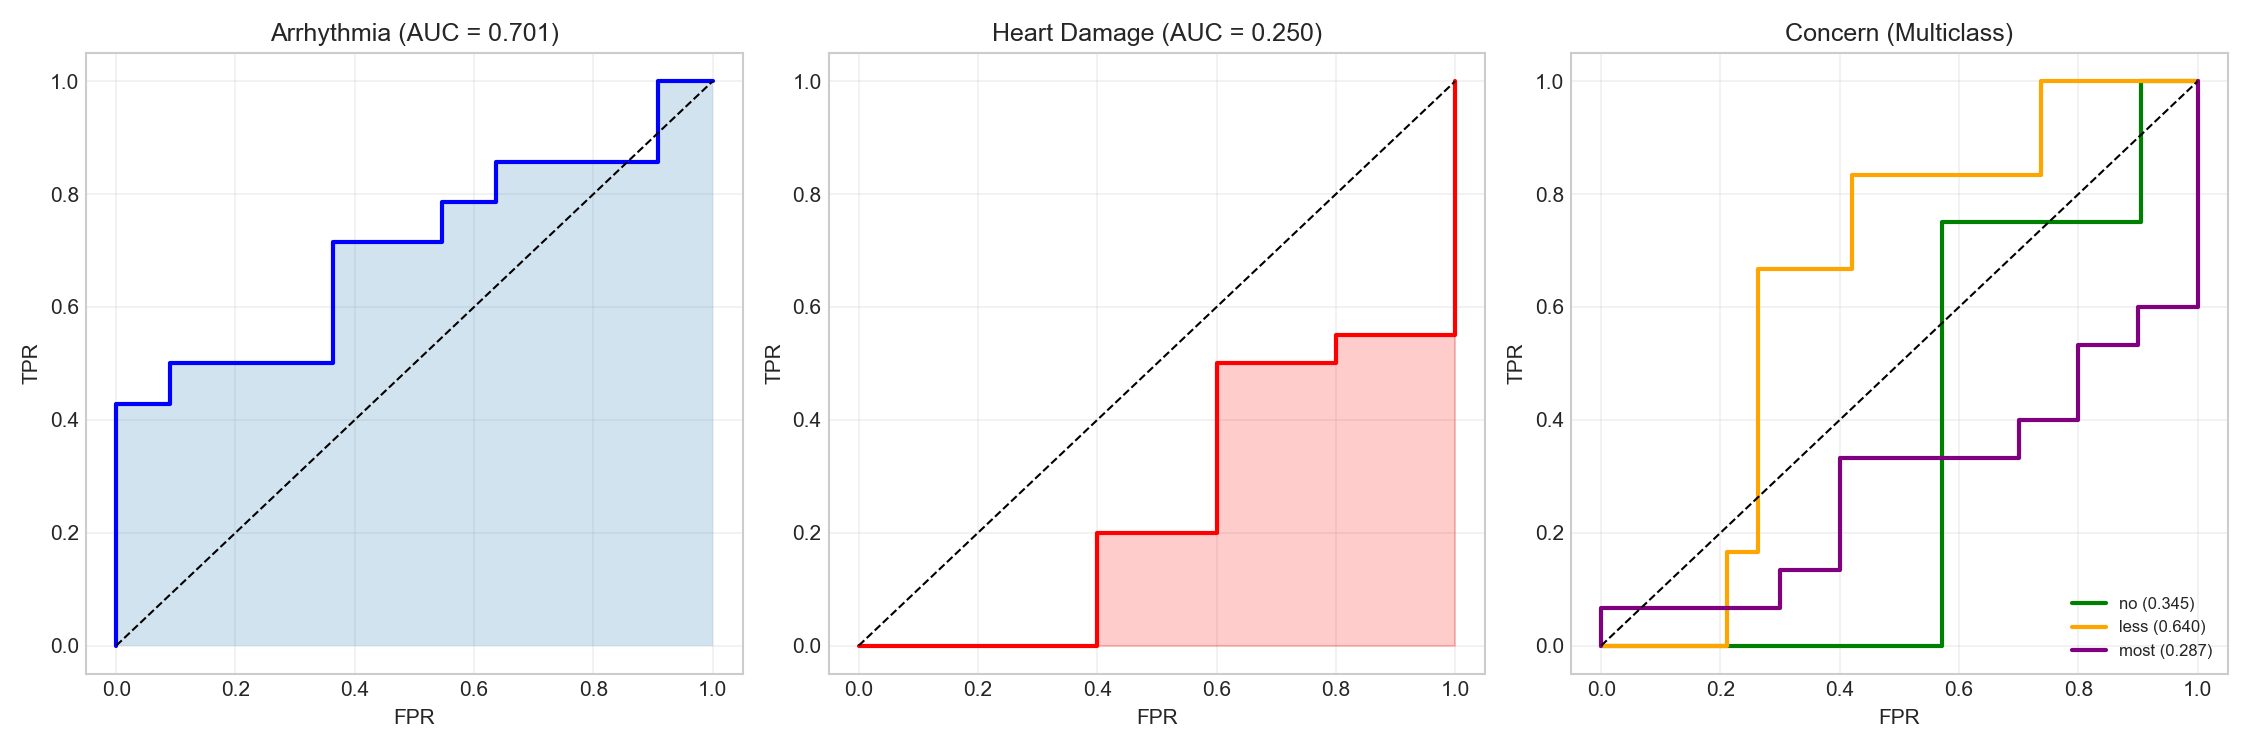
\includegraphics[width=\textwidth]{../Prediction_Plots/summary_roc.png}
\caption{ROC curves for all prediction models.}
\label{fig:roc_summary}
\end{figure}


\subsection{Arrhythmia}

\begin{figure}[H]
\centering

\includegraphics[width=0.7\textwidth]{../Prediction_Plots/roc_arrhythmia.png}
\caption{ROC curve for Arrhythmia prediction.}
\label{fig:roc_arrhythmia}
\end{figure}


\subsection{Heart Damage}

\begin{figure}[H]
\centering

\includegraphics[width=0.7\textwidth]{../Prediction_Plots/roc_heart_damage.png}
\caption{ROC curve for Heart Damage prediction.}
\label{fig:roc_heart_damage}
\end{figure}


\subsection{Concern}

\begin{figure}[H]
\centering
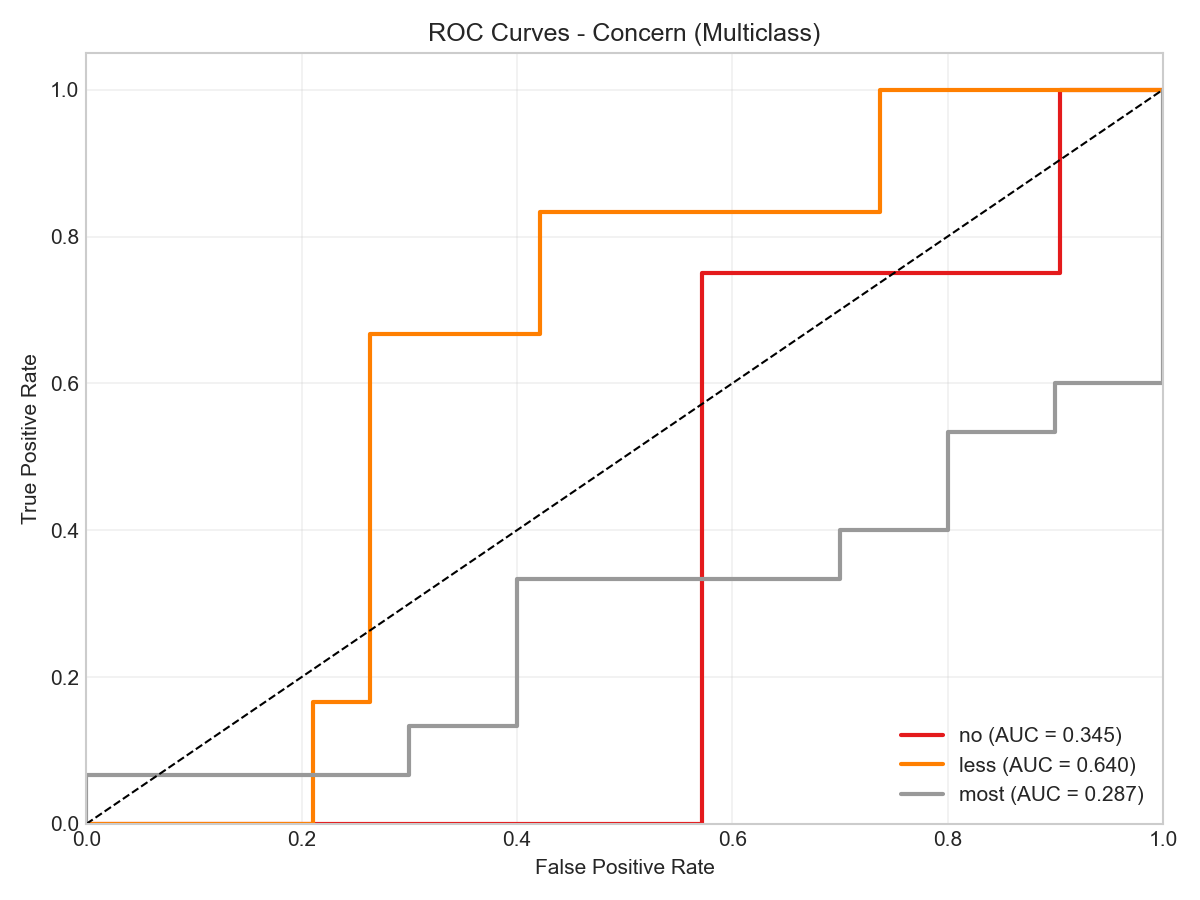
\includegraphics[width=0.7\textwidth]{../Prediction_Plots/roc_concern.png}
\caption{ROC curve for Concern prediction.}
\label{fig:roc_concern}
\end{figure}


\section{Confusion Matrices}


\subsection{Arrhythmia}

\begin{figure}[H]
\centering
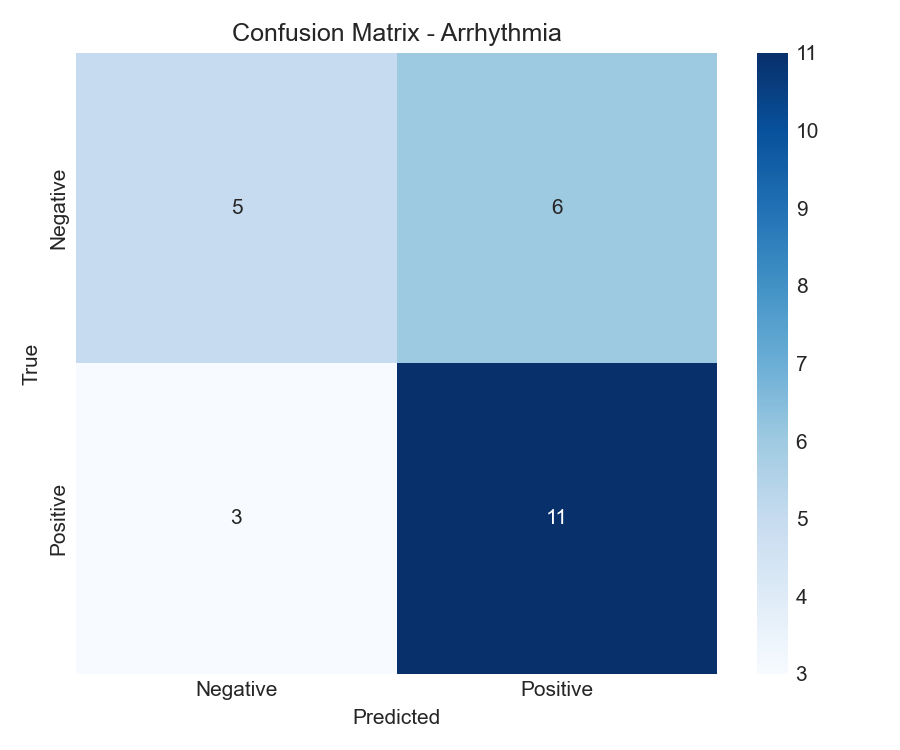
\includegraphics[width=0.5\textwidth]{../Prediction_Plots/cm_arrhythmia.png}
\caption{Confusion matrix for Arrhythmia prediction.}
\label{fig:cm_arrhythmia}
\end{figure}


\subsection{Heart Damage}

\begin{figure}[H]
\centering
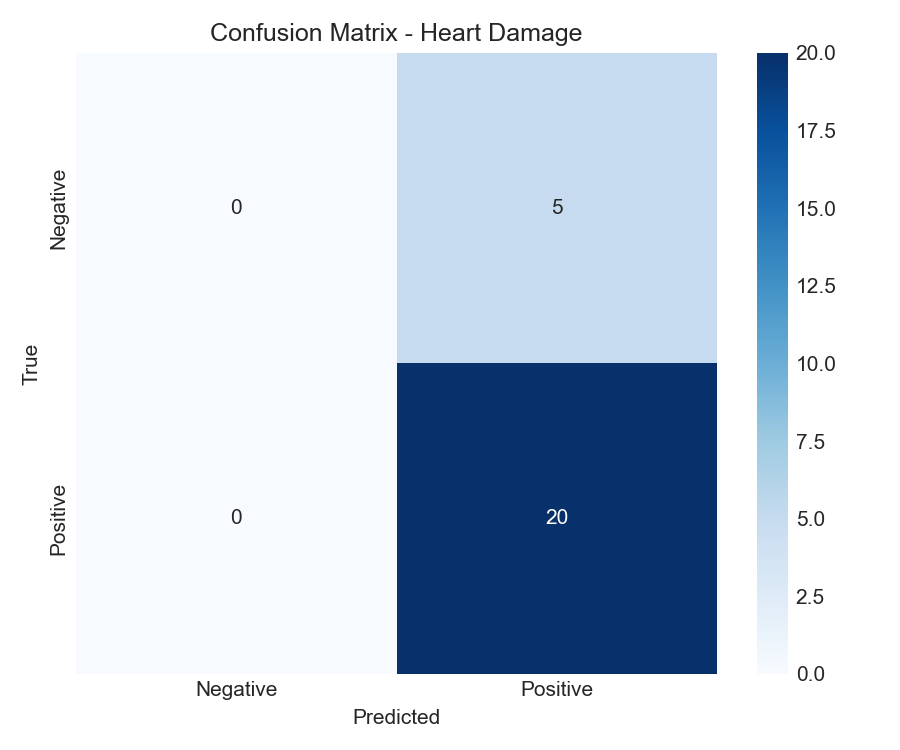
\includegraphics[width=0.5\textwidth]{../Prediction_Plots/cm_heart_damage.png}
\caption{Confusion matrix for Heart Damage prediction.}
\label{fig:cm_heart_damage}
\end{figure}


\subsection{Concern}

\begin{figure}[H]
\centering
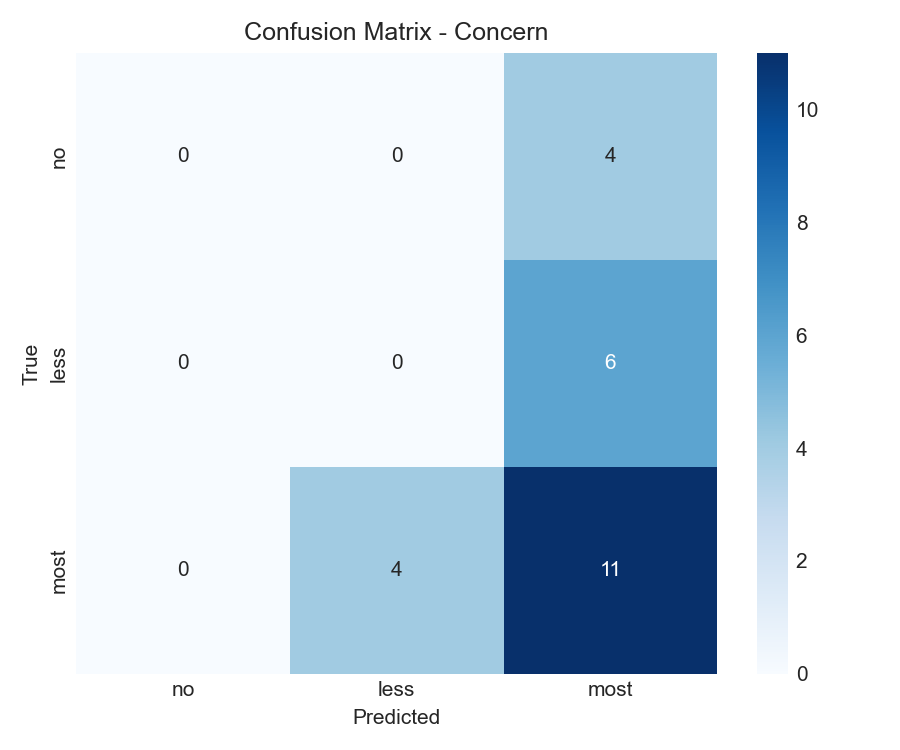
\includegraphics[width=0.5\textwidth]{../Prediction_Plots/cm_concern.png}
\caption{Confusion matrix for Concern prediction.}
\label{fig:cm_concern}
\end{figure}


\section{Feature Importance}


\begin{table}[htbp]
\centering
\caption{Top 10 Most Important Features by Model}
\label{tab:features}
\begin{tabular}{clc}
\toprule
\textbf{Rank} & \textbf{Feature} & \textbf{Importance} \\
\midrule
\multicolumn{3}{c}{\textbf{Arrhythmia}} \\
\midrule
1 & mt\_Contractility & 0.1955 \\
2 & R0\_Contractility & 0.1465 \\
3 & mb\_Contractility & 0.1218 \\
4 & tau\_b\_O2 & 0.0939 \\
5 & tau\_b\_Contractility & 0.0864 \\
6 & A\_tox\_O2 & 0.0790 \\
7 & nb\_Contractility & 0.0776 \\
8 & mb\_O2 & 0.0733 \\
9 & nt\_Contractility & 0.0527 \\
10 & tau\_t\_Contractility & 0.0503 \\
\midrule
\multicolumn{3}{c}{\textbf{Heart Damage}} \\
\midrule
1 & kb\_O2 & 0.0640 \\
2 & nb\_O2 & 0.0600 \\
3 & nb\_Contractility & 0.0560 \\
4 & mb\_O2 & 0.0520 \\
5 & nt\_Contractility & 0.0480 \\
6 & mt\_O2 & 0.0440 \\
7 & tau\_b\_Contractility & 0.0400 \\
8 & R0\_Contractility & 0.0400 \\
9 & A\_tox\_O2 & 0.0400 \\
10 & A\_tox\_Contractility & 0.0360 \\
\midrule
\multicolumn{3}{c}{\textbf{Concern}} \\
\midrule
1 & A\_benefit\_Contractility & 0.1089 \\
2 & nt\_Contractility & 0.1065 \\
3 & A\_tox\_Contractility & 0.0733 \\
4 & tau\_t\_Contractility & 0.0696 \\
5 & kt\_O2 & 0.0582 \\
6 & mb\_Contractility & 0.0580 \\
7 & A\_tox\_O2 & 0.0567 \\
8 & tau\_t\_O2 & 0.0556 \\
9 & kb\_O2 & 0.0529 \\
10 & tau\_b\_Contractility & 0.0526 \\
\midrule

\bottomrule
\end{tabular}
\end{table}

\subsection{Arrhythmia}

\begin{figure}[H]
\centering
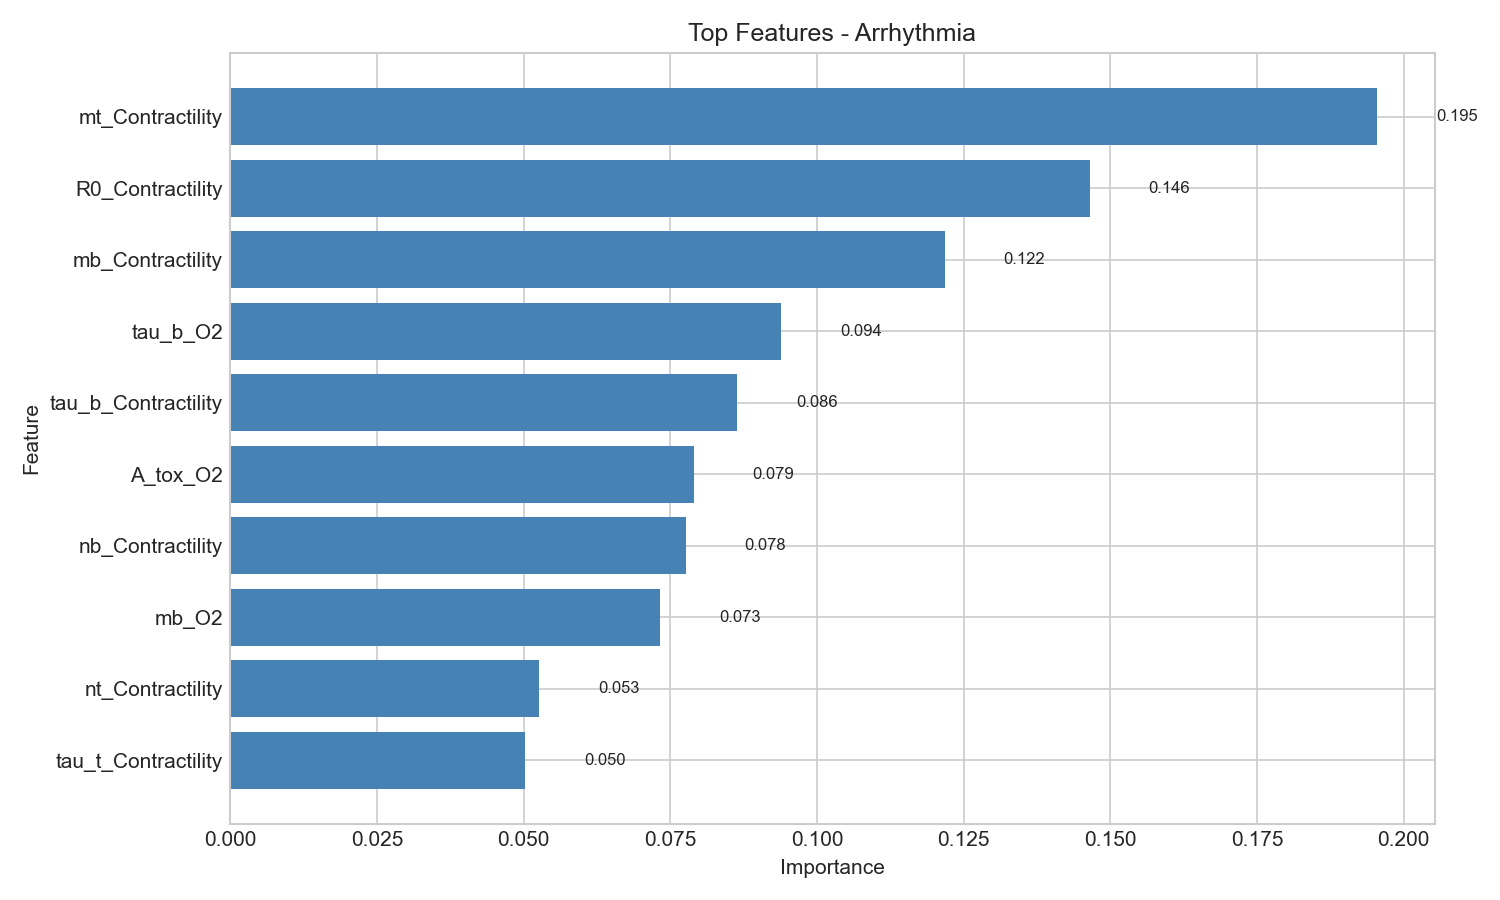
\includegraphics[width=0.8\textwidth]{../Prediction_Plots/importance_arrhythmia.png}
\caption{Top features for Arrhythmia prediction.}
\label{fig:importance_arrhythmia}
\end{figure}


\subsection{Heart Damage}

\begin{figure}[H]
\centering
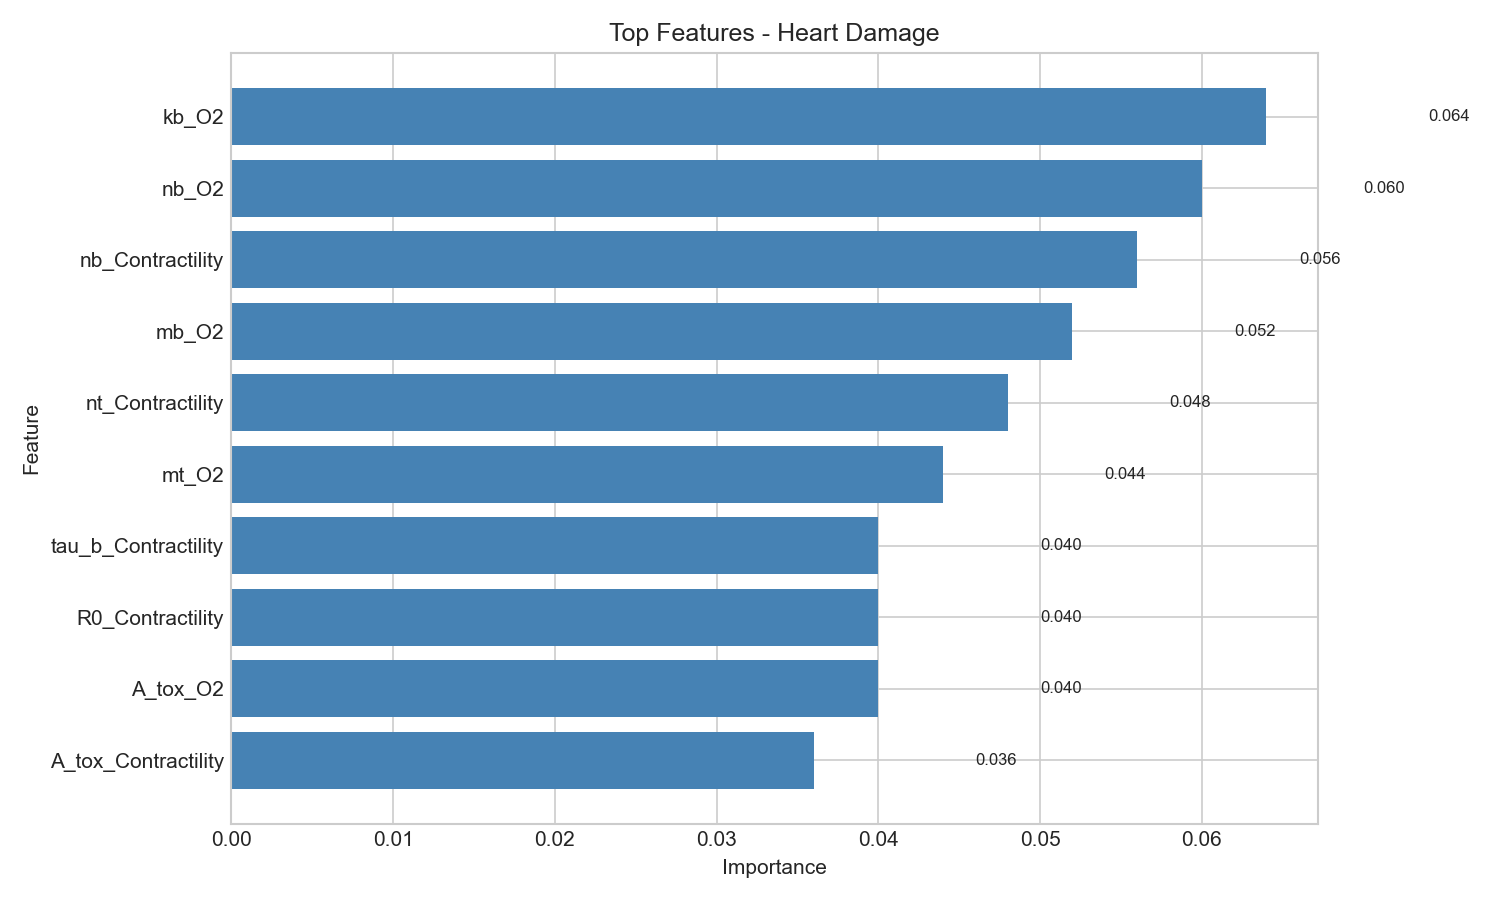
\includegraphics[width=0.8\textwidth]{../Prediction_Plots/importance_heart_damage.png}
\caption{Top features for Heart Damage prediction.}
\label{fig:importance_heart_damage}
\end{figure}


\subsection{Concern}

\begin{figure}[H]
\centering
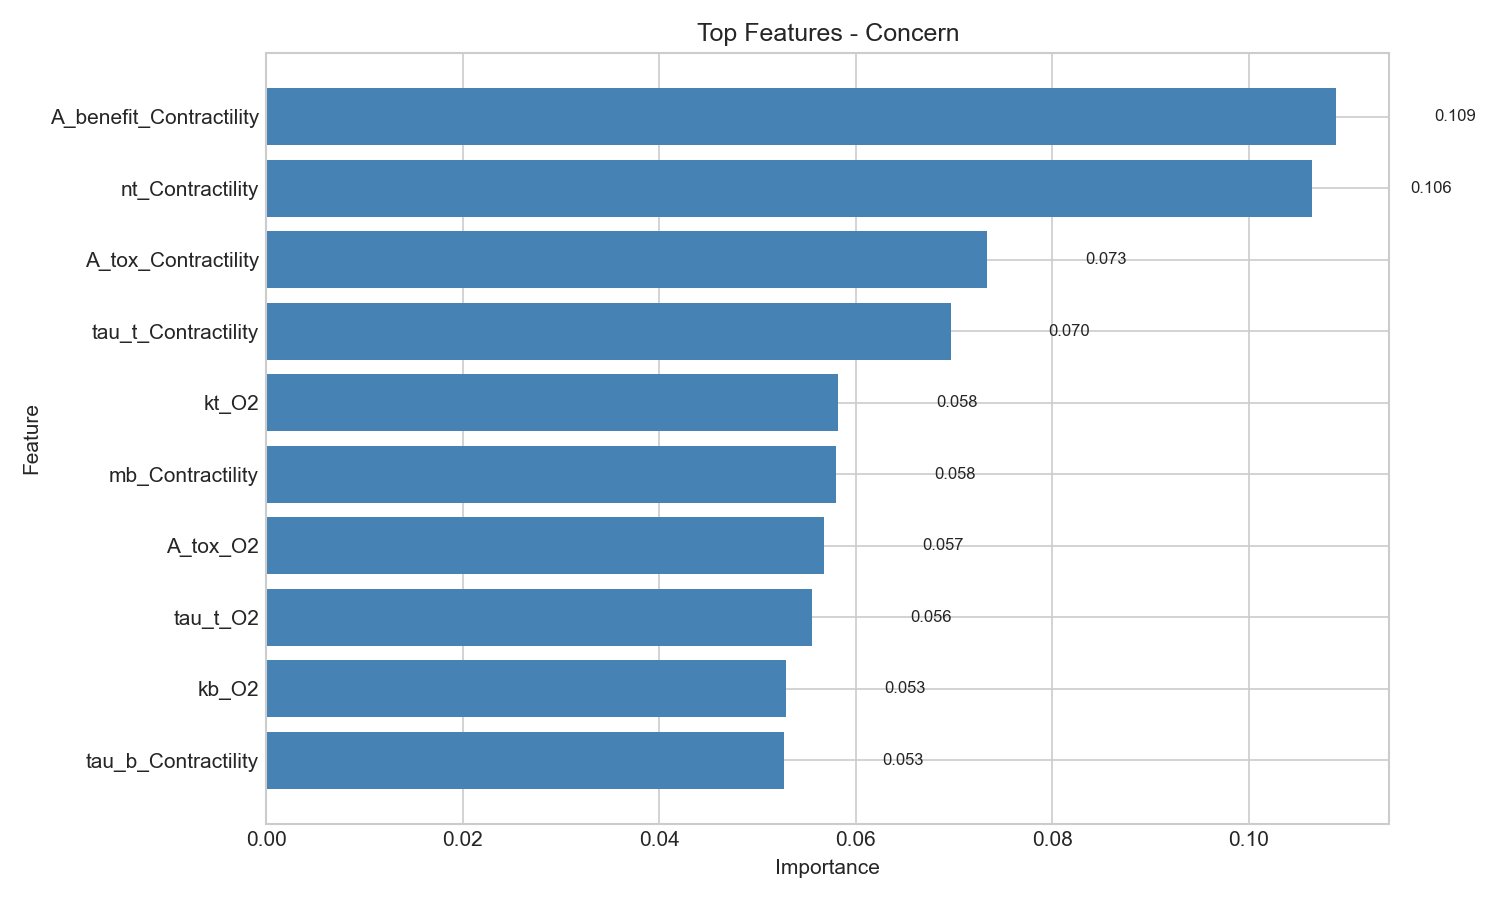
\includegraphics[width=0.8\textwidth]{../Prediction_Plots/importance_concern.png}
\caption{Top features for Concern prediction.}
\label{fig:importance_concern}
\end{figure}


\section{Methods}

\subsection{Data}

Features were extracted from Dual Exponential coefficients
fitted to drug response data. Each drug has coefficients for both Contractility and O2 responses.

\subsection{Models}

\begin{description}
    \item[Arrhythmia (XGBoost)] Gradient boosting with 100 trees, max depth 3, learning rate 0.1
    \item[Heart Damage (RBF SVM)] Radial basis function kernel with C=1.0, gamma='scale'
    \item[Concern (Random Forest)] 100 trees, max depth 5, min samples split 5
\end{description}

\subsection{Cross-Validation}

Leave-One-Out Cross-Validation (LOOCV) was used to evaluate model performance.
Each sample was held out exactly once for testing while the remaining samples were used for training.
This provides an unbiased estimate of generalization performance.

\subsection{Feature Importance}

\begin{description}
    \item[XGBoost] Native feature importance (gain-based)
    \item[RBF SVM] Permutation importance (10 repeats)
    \item[Random Forest] Native feature importance (impurity-based)
\end{description}

\section{Conclusion}

The models demonstrate varying levels of predictive performance across the three cardiac outcomes.
The LOOCV approach ensures robust evaluation on the limited sample size.

\end{document}
